

\tikzset{every picture/.style={line width=0.75pt}} %set default line width to 0.75pt        

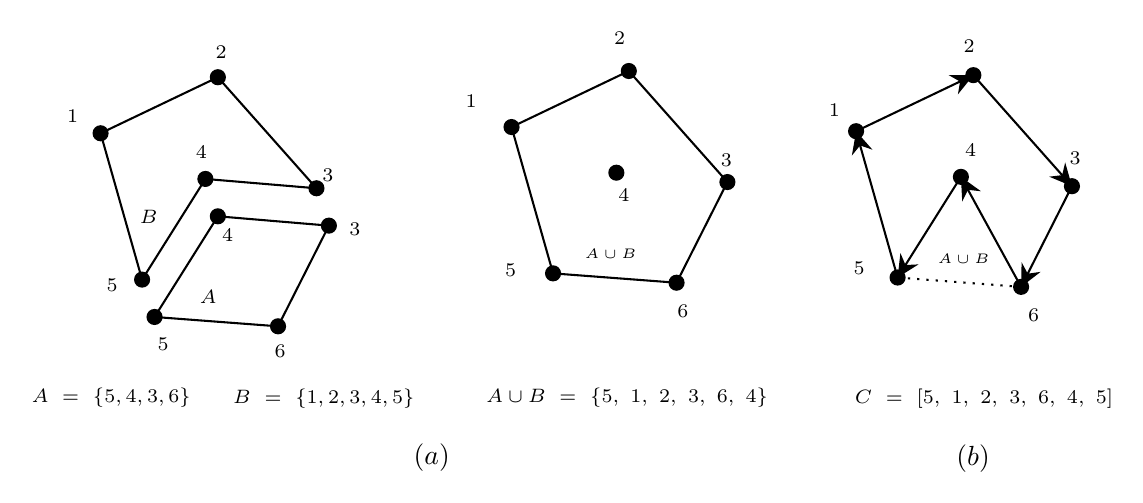
\begin{tikzpicture}[x=0.75pt,y=0.75pt,yscale=-1,xscale=1]
%uncomment if require: \path (0,300); %set diagram left start at 0, and has height of 300

%Shape: Circle [id:dp13697713918046373] 
\draw  [fill={rgb, 255:red, 0; green, 0; blue, 0 }  ,fill opacity=1 ] (84.75,62.38) .. controls (84.75,60.51) and (86.26,59) .. (88.13,59) .. controls (89.99,59) and (91.5,60.51) .. (91.5,62.38) .. controls (91.5,64.24) and (89.99,65.75) .. (88.13,65.75) .. controls (86.26,65.75) and (84.75,64.24) .. (84.75,62.38) -- cycle ;
%Shape: Circle [id:dp8505726277522575] 
\draw  [fill={rgb, 255:red, 0; green, 0; blue, 0 }  ,fill opacity=1 ] (110.75,150.88) .. controls (110.75,149.01) and (112.26,147.5) .. (114.13,147.5) .. controls (115.99,147.5) and (117.5,149.01) .. (117.5,150.88) .. controls (117.5,152.74) and (115.99,154.25) .. (114.13,154.25) .. controls (112.26,154.25) and (110.75,152.74) .. (110.75,150.88) -- cycle ;
%Shape: Circle [id:dp6957030526501801] 
\draw  [fill={rgb, 255:red, 0; green, 0; blue, 0 }  ,fill opacity=1 ] (135.25,84.38) .. controls (135.25,82.51) and (136.76,81) .. (138.63,81) .. controls (140.49,81) and (142,82.51) .. (142,84.38) .. controls (142,86.24) and (140.49,87.75) .. (138.63,87.75) .. controls (136.76,87.75) and (135.25,86.24) .. (135.25,84.38) -- cycle ;
%Shape: Circle [id:dp3439063051120669] 
\draw  [fill={rgb, 255:red, 0; green, 0; blue, 0 }  ,fill opacity=1 ] (188.75,88.88) .. controls (188.75,87.01) and (190.26,85.5) .. (192.13,85.5) .. controls (193.99,85.5) and (195.5,87.01) .. (195.5,88.88) .. controls (195.5,90.74) and (193.99,92.25) .. (192.13,92.25) .. controls (190.26,92.25) and (188.75,90.74) .. (188.75,88.88) -- cycle ;
%Shape: Circle [id:dp9704095790958681] 
\draw  [fill={rgb, 255:red, 0; green, 0; blue, 0 }  ,fill opacity=1 ] (141.25,35.38) .. controls (141.25,33.51) and (142.76,32) .. (144.63,32) .. controls (146.49,32) and (148,33.51) .. (148,35.38) .. controls (148,37.24) and (146.49,38.75) .. (144.63,38.75) .. controls (142.76,38.75) and (141.25,37.24) .. (141.25,35.38) -- cycle ;
%Shape: Circle [id:dp25998291130696727] 
\draw  [fill={rgb, 255:red, 0; green, 0; blue, 0 }  ,fill opacity=1 ] (104.75,132.88) .. controls (104.75,131.01) and (106.26,129.5) .. (108.13,129.5) .. controls (109.99,129.5) and (111.5,131.01) .. (111.5,132.88) .. controls (111.5,134.74) and (109.99,136.25) .. (108.13,136.25) .. controls (106.26,136.25) and (104.75,134.74) .. (104.75,132.88) -- cycle ;
%Shape: Circle [id:dp2350631327028263] 
\draw  [fill={rgb, 255:red, 0; green, 0; blue, 0 }  ,fill opacity=1 ] (141.25,102.38) .. controls (141.25,100.51) and (142.76,99) .. (144.63,99) .. controls (146.49,99) and (148,100.51) .. (148,102.38) .. controls (148,104.24) and (146.49,105.75) .. (144.63,105.75) .. controls (142.76,105.75) and (141.25,104.24) .. (141.25,102.38) -- cycle ;
%Shape: Circle [id:dp7827844033831461] 
\draw  [fill={rgb, 255:red, 0; green, 0; blue, 0 }  ,fill opacity=1 ] (194.75,106.88) .. controls (194.75,105.01) and (196.26,103.5) .. (198.13,103.5) .. controls (199.99,103.5) and (201.5,105.01) .. (201.5,106.88) .. controls (201.5,108.74) and (199.99,110.25) .. (198.13,110.25) .. controls (196.26,110.25) and (194.75,108.74) .. (194.75,106.88) -- cycle ;
%Shape: Circle [id:dp5984519628047641] 
\draw  [fill={rgb, 255:red, 0; green, 0; blue, 0 }  ,fill opacity=1 ] (170.25,155.38) .. controls (170.25,153.51) and (171.76,152) .. (173.63,152) .. controls (175.49,152) and (177,153.51) .. (177,155.38) .. controls (177,157.24) and (175.49,158.75) .. (173.63,158.75) .. controls (171.76,158.75) and (170.25,157.24) .. (170.25,155.38) -- cycle ;
%Straight Lines [id:da06862524702693684] 
\draw    (88.13,62.38) -- (144.63,35.38) ;
%Straight Lines [id:da9660786684329544] 
\draw    (144.63,35.38) -- (192.13,88.88) ;
%Straight Lines [id:da7348457697602903] 
\draw    (138.63,84.38) -- (192.13,88.88) ;
%Straight Lines [id:da4750360942060473] 
\draw    (138.63,84.38) -- (108.13,132.88) ;
%Straight Lines [id:da6122051730873473] 
\draw    (88.13,62.38) -- (108.13,132.88) ;
%Straight Lines [id:da14464697295758544] 
\draw    (144.63,102.38) -- (114.13,150.88) ;
%Straight Lines [id:da30526871036725645] 
\draw    (144.63,102.38) -- (198.13,106.88) ;
%Straight Lines [id:da9282358610345429] 
\draw    (173.63,155.38) -- (114.13,150.88) ;
%Straight Lines [id:da7128692568004056] 
\draw    (173.63,155.38) -- (198.13,106.88) ;
%Shape: Circle [id:dp8591338688223725] 
\draw  [fill={rgb, 255:red, 0; green, 0; blue, 0 }  ,fill opacity=1 ] (282.75,59.38) .. controls (282.75,57.51) and (284.26,56) .. (286.13,56) .. controls (287.99,56) and (289.5,57.51) .. (289.5,59.38) .. controls (289.5,61.24) and (287.99,62.75) .. (286.13,62.75) .. controls (284.26,62.75) and (282.75,61.24) .. (282.75,59.38) -- cycle ;
%Shape: Circle [id:dp44136628753488827] 
\draw  [fill={rgb, 255:red, 0; green, 0; blue, 0 }  ,fill opacity=1 ] (333.25,81.38) .. controls (333.25,79.51) and (334.76,78) .. (336.63,78) .. controls (338.49,78) and (340,79.51) .. (340,81.38) .. controls (340,83.24) and (338.49,84.75) .. (336.63,84.75) .. controls (334.76,84.75) and (333.25,83.24) .. (333.25,81.38) -- cycle ;
%Shape: Circle [id:dp5197915292676696] 
\draw  [fill={rgb, 255:red, 0; green, 0; blue, 0 }  ,fill opacity=1 ] (386.75,85.88) .. controls (386.75,84.01) and (388.26,82.5) .. (390.13,82.5) .. controls (391.99,82.5) and (393.5,84.01) .. (393.5,85.88) .. controls (393.5,87.74) and (391.99,89.25) .. (390.13,89.25) .. controls (388.26,89.25) and (386.75,87.74) .. (386.75,85.88) -- cycle ;
%Shape: Circle [id:dp2805204502688967] 
\draw  [fill={rgb, 255:red, 0; green, 0; blue, 0 }  ,fill opacity=1 ] (339.25,32.38) .. controls (339.25,30.51) and (340.76,29) .. (342.63,29) .. controls (344.49,29) and (346,30.51) .. (346,32.38) .. controls (346,34.24) and (344.49,35.75) .. (342.63,35.75) .. controls (340.76,35.75) and (339.25,34.24) .. (339.25,32.38) -- cycle ;
%Shape: Circle [id:dp8899258705918431] 
\draw  [fill={rgb, 255:red, 0; green, 0; blue, 0 }  ,fill opacity=1 ] (302.75,129.88) .. controls (302.75,128.01) and (304.26,126.5) .. (306.13,126.5) .. controls (307.99,126.5) and (309.5,128.01) .. (309.5,129.88) .. controls (309.5,131.74) and (307.99,133.25) .. (306.13,133.25) .. controls (304.26,133.25) and (302.75,131.74) .. (302.75,129.88) -- cycle ;
%Shape: Circle [id:dp4722303212665844] 
\draw  [fill={rgb, 255:red, 0; green, 0; blue, 0 }  ,fill opacity=1 ] (362.25,134.38) .. controls (362.25,132.51) and (363.76,131) .. (365.63,131) .. controls (367.49,131) and (369,132.51) .. (369,134.38) .. controls (369,136.24) and (367.49,137.75) .. (365.63,137.75) .. controls (363.76,137.75) and (362.25,136.24) .. (362.25,134.38) -- cycle ;
%Straight Lines [id:da8779034684774795] 
\draw    (286.13,59.38) -- (342.63,32.38) ;
%Straight Lines [id:da5866163501693322] 
\draw    (342.63,32.38) -- (390.13,85.88) ;
%Straight Lines [id:da20891965910292054] 
\draw    (286.13,59.38) -- (306.13,129.88) ;
%Straight Lines [id:da4480795127777464] 
\draw    (365.63,134.38) -- (306.13,129.88) ;
%Straight Lines [id:da4030448761724379] 
\draw    (365.63,134.38) -- (390.13,85.88) ;
%Shape: Circle [id:dp12505357057171118] 
\draw  [fill={rgb, 255:red, 0; green, 0; blue, 0 }  ,fill opacity=1 ] (448.75,61.38) .. controls (448.75,59.51) and (450.26,58) .. (452.13,58) .. controls (453.99,58) and (455.5,59.51) .. (455.5,61.38) .. controls (455.5,63.24) and (453.99,64.75) .. (452.13,64.75) .. controls (450.26,64.75) and (448.75,63.24) .. (448.75,61.38) -- cycle ;
%Shape: Circle [id:dp5746788054186597] 
\draw  [fill={rgb, 255:red, 0; green, 0; blue, 0 }  ,fill opacity=1 ] (499.25,83.38) .. controls (499.25,81.51) and (500.76,80) .. (502.63,80) .. controls (504.49,80) and (506,81.51) .. (506,83.38) .. controls (506,85.24) and (504.49,86.75) .. (502.63,86.75) .. controls (500.76,86.75) and (499.25,85.24) .. (499.25,83.38) -- cycle ;
%Shape: Circle [id:dp09128011464267372] 
\draw  [fill={rgb, 255:red, 0; green, 0; blue, 0 }  ,fill opacity=1 ] (552.75,87.88) .. controls (552.75,86.01) and (554.26,84.5) .. (556.13,84.5) .. controls (557.99,84.5) and (559.5,86.01) .. (559.5,87.88) .. controls (559.5,89.74) and (557.99,91.25) .. (556.13,91.25) .. controls (554.26,91.25) and (552.75,89.74) .. (552.75,87.88) -- cycle ;
%Shape: Circle [id:dp4758380405926569] 
\draw  [fill={rgb, 255:red, 0; green, 0; blue, 0 }  ,fill opacity=1 ] (505.25,34.38) .. controls (505.25,32.51) and (506.76,31) .. (508.63,31) .. controls (510.49,31) and (512,32.51) .. (512,34.38) .. controls (512,36.24) and (510.49,37.75) .. (508.63,37.75) .. controls (506.76,37.75) and (505.25,36.24) .. (505.25,34.38) -- cycle ;
%Shape: Circle [id:dp46268099577976185] 
\draw  [fill={rgb, 255:red, 0; green, 0; blue, 0 }  ,fill opacity=1 ] (468.75,131.88) .. controls (468.75,130.01) and (470.26,128.5) .. (472.13,128.5) .. controls (473.99,128.5) and (475.5,130.01) .. (475.5,131.88) .. controls (475.5,133.74) and (473.99,135.25) .. (472.13,135.25) .. controls (470.26,135.25) and (468.75,133.74) .. (468.75,131.88) -- cycle ;
%Shape: Circle [id:dp29163272981610444] 
\draw  [fill={rgb, 255:red, 0; green, 0; blue, 0 }  ,fill opacity=1 ] (528.25,136.38) .. controls (528.25,134.51) and (529.76,133) .. (531.63,133) .. controls (533.49,133) and (535,134.51) .. (535,136.38) .. controls (535,138.24) and (533.49,139.75) .. (531.63,139.75) .. controls (529.76,139.75) and (528.25,138.24) .. (528.25,136.38) -- cycle ;
%Straight Lines [id:da32662852992492064] 
\draw    (452.13,61.38) -- (505.92,35.67) ;
\draw [shift={(508.63,34.38)}, rotate = 154.46] [fill={rgb, 255:red, 0; green, 0; blue, 0 }  ][line width=0.08]  [draw opacity=0] (10.72,-5.15) -- (0,0) -- (10.72,5.15) -- (7.12,0) -- cycle    ;
%Straight Lines [id:da7621252383734732] 
\draw    (508.63,34.38) -- (554.13,85.63) ;
\draw [shift={(556.13,87.88)}, rotate = 228.4] [fill={rgb, 255:red, 0; green, 0; blue, 0 }  ][line width=0.08]  [draw opacity=0] (10.72,-5.15) -- (0,0) -- (10.72,5.15) -- (7.12,0) -- cycle    ;
%Straight Lines [id:da6231835233611202] 
\draw    (502.63,83.38) -- (473.72,129.34) ;
\draw [shift={(472.13,131.88)}, rotate = 302.16] [fill={rgb, 255:red, 0; green, 0; blue, 0 }  ][line width=0.08]  [draw opacity=0] (10.72,-5.15) -- (0,0) -- (10.72,5.15) -- (7.12,0) -- cycle    ;
%Straight Lines [id:da5474926953011492] 
\draw    (452.94,64.26) -- (472.13,131.88) ;
\draw [shift={(452.13,61.38)}, rotate = 74.16] [fill={rgb, 255:red, 0; green, 0; blue, 0 }  ][line width=0.08]  [draw opacity=0] (10.72,-5.15) -- (0,0) -- (10.72,5.15) -- (7.12,0) -- cycle    ;
%Straight Lines [id:da651840469987403] 
\draw  [dash pattern={on 0.84pt off 2.51pt}]  (531.63,136.38) -- (472.13,131.88) ;
%Straight Lines [id:da6912887937841965] 
\draw    (532.98,133.7) -- (556.13,87.88) ;
\draw [shift={(531.63,136.38)}, rotate = 296.8] [fill={rgb, 255:red, 0; green, 0; blue, 0 }  ][line width=0.08]  [draw opacity=0] (10.72,-5.15) -- (0,0) -- (10.72,5.15) -- (7.12,0) -- cycle    ;
%Straight Lines [id:da3792915173272351] 
\draw    (504.07,86.01) -- (531.63,136.38) ;
\draw [shift={(502.63,83.38)}, rotate = 61.31] [fill={rgb, 255:red, 0; green, 0; blue, 0 }  ][line width=0.08]  [draw opacity=0] (10.72,-5.15) -- (0,0) -- (10.72,5.15) -- (7.12,0) -- cycle    ;

% Text Node
\draw (262.5,42.5) node [anchor=north west][inner sep=0.75pt]  [font=\scriptsize] [align=left] {1};
% Text Node
\draw (281.5,124) node [anchor=north west][inner sep=0.75pt]  [font=\scriptsize] [align=left] {5};
% Text Node
\draw (132.5,67) node [anchor=north west][inner sep=0.75pt]  [font=\scriptsize] [align=left] {4};
% Text Node
\draw (385.5,71) node [anchor=north west][inner sep=0.75pt]  [font=\scriptsize] [align=left] {3};
% Text Node
\draw (334,12) node [anchor=north west][inner sep=0.75pt]  [font=\scriptsize] [align=left] {2};
% Text Node
\draw (336.13,87.88) node [anchor=north west][inner sep=0.75pt]  [font=\scriptsize] [align=left] {4};
% Text Node
\draw (206.5,104) node [anchor=north west][inner sep=0.75pt]  [font=\scriptsize] [align=left] {3};
% Text Node
\draw (364.5,143.5) node [anchor=north west][inner sep=0.75pt]  [font=\scriptsize] [align=left] {6};
% Text Node
\draw (114.13,159.38) node [anchor=north west][inner sep=0.75pt]  [font=\scriptsize] [align=left] {5};
% Text Node
\draw (437.5,47) node [anchor=north west][inner sep=0.75pt]  [font=\scriptsize] [align=left] {1};
% Text Node
\draw (449.5,123) node [anchor=north west][inner sep=0.75pt]  [font=\scriptsize] [align=left] {5};
% Text Node
\draw (553.5,70) node [anchor=north west][inner sep=0.75pt]  [font=\scriptsize] [align=left] {3};
% Text Node
\draw (502.5,16) node [anchor=north west][inner sep=0.75pt]  [font=\scriptsize] [align=left] {2};
% Text Node
\draw (503.13,66.25) node [anchor=north west][inner sep=0.75pt]  [font=\scriptsize] [align=left] {4};
% Text Node
\draw (533.5,145.5) node [anchor=north west][inner sep=0.75pt]  [font=\scriptsize] [align=left] {6};
% Text Node
\draw (70.5,49.5) node [anchor=north west][inner sep=0.75pt]  [font=\scriptsize] [align=left] {1};
% Text Node
\draw (89.5,131) node [anchor=north west][inner sep=0.75pt]  [font=\scriptsize] [align=left] {5};
% Text Node
\draw (193.5,78) node [anchor=north west][inner sep=0.75pt]  [font=\scriptsize] [align=left] {3};
% Text Node
\draw (142,19) node [anchor=north west][inner sep=0.75pt]  [font=\scriptsize] [align=left] {2};
% Text Node
\draw (145.13,106.88) node [anchor=north west][inner sep=0.75pt]  [font=\scriptsize] [align=left] {4};
% Text Node
\draw (170.5,163) node [anchor=north west][inner sep=0.75pt]  [font=\scriptsize] [align=left] {6};
% Text Node
\draw (134.5,136.5) node [anchor=north west][inner sep=0.75pt]  [font=\scriptsize] [align=left] {$\displaystyle A$};
% Text Node
\draw (105.5,98) node [anchor=north west][inner sep=0.75pt]  [font=\scriptsize] [align=left] {$\displaystyle B$};
% Text Node
\draw (490,119) node [anchor=north west][inner sep=0.75pt]  [font=\tiny] [align=left] {$\displaystyle A\cup B$};
% Text Node
\draw (320,116.5) node [anchor=north west][inner sep=0.75pt]  [font=\tiny] [align=left] {$\displaystyle A\cup B$};
% Text Node
\draw (53.5,183.5) node [anchor=north west][inner sep=0.75pt]  [font=\scriptsize] [align=left] {$\displaystyle A\ =\ \{5,4,3,6\}$};
% Text Node
\draw (150.5,184) node [anchor=north west][inner sep=0.75pt]  [font=\scriptsize] [align=left] {$\displaystyle B\ =\ \{1,2,3,4,5\}$};
% Text Node
\draw (272.5,183.5) node [anchor=north west][inner sep=0.75pt]  [font=\scriptsize] [align=left] {$\displaystyle A\cup B\ =\ \{5,\ 1,\ 2,\ 3,\ 6,\ 4\}$};
% Text Node
\draw (450,184) node [anchor=north west][inner sep=0.75pt]  [font=\scriptsize] [align=left] {$\displaystyle C\ =\ [ 5,\ 1,\ 2,\ 3,\ 6,\ 4,\ 5]$};
% Text Node
\draw (237.5,210.5) node [anchor=north west][inner sep=0.75pt]   [align=left] {$\displaystyle ( a)$};
% Text Node
\draw (499,211) node [anchor=north west][inner sep=0.75pt]   [align=left] {$\displaystyle ( b)$};


\end{tikzpicture}
